\documentclass[svgnames,11pt]{standalone}
\usepackage[utf8]{inputenc}
\usepackage[T1]{fontenc}
\usepackage{csquotes}
\usepackage[english]{babel}
\usepackage{xcolor}
\usepackage{charter}
\usepackage{amsmath}
\usepackage{amssymb}
\usepackage[np,autolanguage]{numprint}
\newcommand{\outqt}[1]{{\textcolor{DarkOrange}{#1}}}
\newcommand{\inqt}[1]{{\textcolor{Blue}{#1}}}
\usepackage{tikz}
\usetikzlibrary{arrows,automata,calc}
\usetikzlibrary{arrows.meta}
\usetikzlibrary{decorations.pathreplacing}
\usetikzlibrary{backgrounds,shapes}
\tikzset{%
  show curve controls/.style={
    postaction={
      decoration={
        show path construction,
        curveto code={
          \draw [blue] 
            (\tikzinputsegmentfirst) -- (\tikzinputsegmentsupporta)
            (\tikzinputsegmentlast) -- (\tikzinputsegmentsupportb);
          \fill [red, opacity=0.5] 
            (\tikzinputsegmentsupporta) circle [radius=.25ex]
            (\tikzinputsegmentsupportb) circle [radius=.25ex];
        }
      },
      decorate
}}}
\tikzstyle{vertex}=[draw,circle,black,inner sep=2pt]
\tikzstyle{edge}=[line width=1.3pt,color=Black]
\tikzstyle{rare}=[fill=black,text=white]
\tikzstyle{medium}=[fill=black!15!white]


\begin{document}
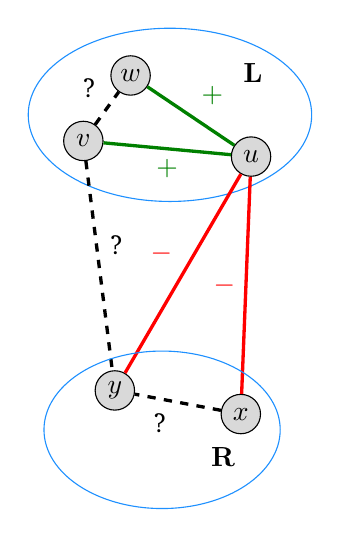
\begin{tikzpicture}[auto,vertex/.append style={minimum width=5mm},
  edge/.append style={line width=1.2pt,color=Black}]

  \node[vertex,medium,] (w) at (0.000, -0.000) {$w$};
  \node[vertex,medium,] (v) at (-.60, -.8315) {$v$};
  \node[vertex,medium,] (u) at (1.53, -1.03) {$u$};

  \draw[edge,Green] (w) -- node [] {$+$} (u) ;
  \draw[edge,Green] (v) -- node [below] {$+$} (u) ;
  \draw[edge,dashed] (v) -- node [] {?} (w) ;

  \draw[color=DodgerBlue] (.5, -.5) circle [x radius=1.8, y radius=1.1]  node[xshift=30, yshift=15,text=Black] {$\mathbf{L}$};

  \node[vertex,medium,] (y) at (-0.200, -4.000) {$y$};
  \node[vertex,medium,] (x) at (1.400, -4.300) {$x$};
  \draw[edge,dashed] (x) -- node [] {?} (y) ;

  \draw[edge,dashed] (v) -- node [] {?} (y) ;

  \draw[edge,Red] (y) -- node [] {$-$} (u) ;
  \draw[edge,Red] (x) -- node [] {$-$} (u) ;

  \draw[color=DodgerBlue] (.4, -4.5) circle [x radius=1.5, y radius=1]  node[xshift=22, yshift=-10,text=Black] {$\mathbf{R}$};


\end{tikzpicture}
\end{document}
